\chapter{线性代数基础}\label{chap:linear-algebra}

\section{线性空间}

从动机上说,线性空间试图将$\R^n$或者$\C^n$这样的集合连同他们上面的代数结构抽象出来. 除此之外,函数和无穷数列的集合也是非常重要的对象,比如说$\R$上的连续函数组成的集合$C(\R)$,或者具有“模长”的无穷复数列($\ell^2$-空间):
\[\ell^2=\left\{x=(x_1,x_2,\cdots)\in\C^\infty:\sum_{i=1}^\infty x_i^2<\infty\right\}.\]

我们将这些对象的共性抽象出来,得到线性空间的概念. 线性空间都是基于某个域定义的,我们先给出域的定义. 

\begin{definition}[域]\index{域}
一个\textbf{域}是一个集合$F$,其上定义了两种二元运算:加法$+$和乘法$\cdot$,他们都是$F\times F$到$F$的映射,满足下面的公理:
\begin{enumerate}
    \item (结合律)对于任意的$a,b,c\in F$,有$(a+b)+c=a+(b+c)$和$(a\cdot b)\cdot c=a\cdot (b\cdot c)$;
    \item (交换律)对于任意的$a,b\in F$,有$a+b=b+a$和$a\cdot b=b\cdot a$;
    \item(分配律)对于任意的$a,b,c\in F$,有$a\cdot(b+c)=a\cdot b+a\cdot c$. 
    \item (单位元)存在唯一的两个元素$0,1\in F$,使得对于任意的$a\in F$,有$a+0=a$和$a\cdot 1=a$;
    \item (加法逆元)对于任意的$a\in F$,存在唯一$b\in F$,使得$a+b=0$,记$b$作$-a$;
    \item (乘法逆元)对于任意的$a\in F$,如果$a\neq 0$,则存在唯一$b\in F$,使得$a\cdot b=1$,记$b$作$a^{-1}$;
\end{enumerate}
通常将$a\cdot b$写作$ab$,并且乘法的优先级高于加法,即$ab+c=(ab)+c$. 
\end{definition}

域的重要例子包括有理数域$\Q$,实数域$\R$和复数域$\C$,他们都是无限域. 我们将在后面的内容中使用这些域. 

\begin{definition}[线性空间,向量空间]\index{线性空间}\index{向量空间}
设$V$是一个集合,$F$是一个域. 如果在$V$上定义了两种运算:加法$+$和数乘$\cdot$,使得$V$满足下面的公理:
\begin{enumerate}
    \item ($V$的结合律)对于任意的$x,y,z\in V$,有$(x+y)+z=x+(y+z)$;
    \item ($V$的交换律)对于任意的$x,y\in V$,有$x+y=y+x$;
    \item (加法零元)存在唯一的元素$0\in V$,使得对于任意的$x\in V$,有$x+0=x$;
    \item (加法逆元)对于任意的$x\in V$,存在唯一$y\in V$,使得$x+y=0$,记$y$作$-x$;
    \item 对于任意的$x\in V$,有$1\cdot x=x$;
    \item 对于任意的$a,b\in F$和$x\in V$,有$(ab)\cdot x=a\cdot (b\cdot x)$;
    \item 对于任意的$a\in F$和$x,y\in V$,有$a\cdot(x+y)=a\cdot x+a\cdot y$;
    \item 对于任意的$a,b\in F$和$x\in V$,有$(a+b)\cdot x=a\cdot x+b\cdot x$. 
\end{enumerate}
则称$V$是一个\textbf{$F$-线性空间},简称\textbf{线性空间},也称\textbf{向量空间}. $V$中的元素被称为\textbf{向量}\index{向量}. 通常将数乘$a\cdot x$写作$ax$,并且乘法的优先级高于加法,即$a\cdot x+y=(a\cdot x)+y$. 
\end{definition}

“线性”一词的含义是指的$ax+by$这种形式的数学对象,线性代数就是研究这种对象的学科. 线性空间的典型例子包括:
\begin{itemize}
    \item $\R^n$和$\C^n$.
    \item $M_{m\times n}(F)$,即所有$m\times n$矩阵组成的集合.
    \item $C(\R)$,即$\R$上的连续函数组成的集合.
    \item $C^k(\R)$,即$\R$上的$k$次连续可微函数组成的集合.
    \item $\ell^2$,即所有二次可和的复数序列组成的集合.
\end{itemize}

如同所有其他的代数结构,线性空间也有各式各样构造新的线性空间的方法. 为了看出来线性空间本质的特性,我们有如下引理:

\begin{lemma}\label{lemma:linear-space-subspace}
设$V$是$F$-线性空间,$W$是$V$的一个子集. 则$W$是一个线性空间当且仅当对任意$a,b\in F$和$x,y\in W$,有$ax+by\in W$. 
\end{lemma}
\begin{proof}
    按照定义即可验证. 
\end{proof}

我们给$ax+by$这样的对象一个正式的定义. 

\begin{definition}[线性组合]\index{线性组合}
设$V$是$F$-线性空间,$x_1,\cdots,x_n\in V$,$a_1,\cdots,a_n\in F$,则称$a_1x_1+\cdots+a_nx_n$是$x_1,\cdots,x_n$的一个\textbf{线性组合}. 
\end{definition}

接下来,基于某些特定的线性空间,我们构造各种新的线性空间. 

\begin{definition}[线性子空间]\index{线性子空间}
设$V$是$F$-线性空间,$W$是$V$的一个子集. 如果$W$是一个线性空间,则称$W$是$V$的一个\textbf{线性子空间}. 
\end{definition}

例如,$\Q$是$\R$的一个线性子空间,但$\Z$不是$\R$的一个线性子空间. 再比如,当$k<l$,$C^k(\R)$是$C^l(\R)$的一个线性子空间. 

\begin{definition}[乘积空间]\index{乘积空间}
设$V_1,\cdots,V_n$是$F$-线性空间,则$V_1\times\cdots\times V_n$是一个$F$-线性空间,其中加法和数乘分别定义为
\begin{align*}
    &(x_1,\cdots,x_n)+(y_1,\cdots,y_n)=(x_1+y_1,\cdots,x_n+y_n),\\
    &a(x_1,\cdots,x_n)=(ax_1,\cdots,ax_n).
\end{align*}
\end{definition}

例如,$\R^n$就是$n$个$\R$的乘积空间,$M_{m\times n}(F)$就是$m\times n$个$F$的乘积空间. 

接下来,我们按照\emph{表示论}\index{表示论}的观点,引入基的概念. 线性空间是一个非常抽象的数学概念,因此我们需要一些具体的元素去表示这整个空间. 

\begin{definition}[生成集]\index{生成集}
设$V$是$F$-线性空间,$S\subseteq V$,如果$V$中的每一个元素都是$S$的线性组合,则称$S$是$V$的一个\textbf{生成集}. 

更一般地,任意一个$S\subseteq V$,我们可以定义 \textbf{$S$生成的线性子空间}为所有$S$的线性组合的集合,记为$\Span(S)$. 
\end{definition}

我们希望用尽可能少的元素来表示整个线性空间,为此,我们需要把“可表示”这样的概念严格化. 

\begin{definition}[线性相关]\index{线性相关}
设$V$是$F$-线性空间,$S\subseteq V$,如果存在$x_1,\cdots,x_n\in S$,$a_1,\cdots,a_n\in F$,使得$a_1x_1+\cdots+a_nx_n=0$,且至少有一个$a_i\neq 0$,则称$S$是\textbf{线性相关}的,否则称$S$是\textbf{线性无关}的. 
\end{definition}

$S$线性相关意味着$S$中的一些元素可以被另一些元素的线性组合表示出来,因而$S$中有一些冗余. 线性无关意味着$S$中的元素都是必要的,没有冗余. 由此,我们可以给出基的定义. 

\begin{definition}[基]\index{基}
设$V$是$F$-线性空间,$S\subseteq V$,如果$S$是线性无关的,并且$\Span(S)=V$,则称$S$是$V$的一个\textbf{基}. 
\end{definition}

线性空间的一个核心定理是基的存在性定理. 

\begin{theorem}[基的存在性定理]\label{thm:existence-of-basis}
设$V$是$F$-线性空间,则$V$中存在一个基. 
\end{theorem}

要注意,这一定理并不是平凡的. 首先,基是线性无关的集合,所以$V$本身通常就不是基. 此外,这一定理要求有一个线性无关的集合$S\subseteq V$,任意向量$x\in V$都可以用$S$中\emph{有限个}元素的线性组合来表示,这样的$S$并不容易找到. 该定理的证明是构造性的,这一构造依赖于选择公理(或者Zorn引理),我们在此略去. 

基的典型例子包括:
\begin{itemize}
    \item $\R^n$的标准基是$\{e_1,\cdots,e_n\}$,其中$e_i$是第$i$个分量为$1$,其余分量为$0$的向量. 
    \item 特别地,$\R$的基就是$\{1\}$,一般地,域$F$作为线性空间的时候,其基就是$\{1\}$. 但如果我们把$\C$看成$\R$的线性空间,那么$\C$的基就是$\{1,i\}$.
    \item $M_{m\times n}(F)$的标准基是$\{E_{ij}:1\leq i\leq m,1\leq j\leq n\}$,其中$E_{ij}$是第$i$行第$j$列为$1$,其余元素为$0$的矩阵. 
    \item $\ell^2$的标准基是$\{e_1,e_2,\cdots\}$,其中$e_i$是第$i$个分量为$1$,其余分量为$0$的实数列. 
\end{itemize}

给定一个基,我们可以用基来表示线性空间中的元素,容易证明,这一表示是唯一的. 因此,我们可以把线性空间中的元素看成基的线性组合,因而有了下面的定义. 

\begin{definition}[坐标]\index{坐标}
设$V$是$F$-线性空间,$S$是$V$的一个基,$x\in V$,如果$x=\sum_{v\in S} a_v v$,则称$(a_v)_{v\in S}$是$x$在基$S$下的\textbf{坐标}. 特别地,如果$S$是有限集,那么$(a_v)_{v\in S}$是一个有限元组,我们也称其为$x$在基$S$下的坐标. 
\end{definition}

例如,$\R^3$的标准基是$\{e_1,e_2,e_3\}$,那么任意$x\in\R^3$都可以表示为$x=a_1e_1+a_2e_2+a_3e_3$,其中$a_i$是$x$的第$i$个分量. 因此,我们可以把$x$看成一个三元组$(a_1,a_2,a_3)$,这就是$x$在标准基下的坐标. 这样的讨论也适用于$\R^n$或$\C^n$. 另外,坐标本身的集合也可以被看作是一个线性空间,例如,$\R^3$的坐标集合就是$\R^3$本身. 

线性空间的基可以衡量线性空间的复杂程度,基元素越少,线性空间越简单. 我们可以定义维数来衡量线性空间的复杂程度. 

\begin{definition}[维数]\index{维数}
设$V$是$F$-线性空间,如果$V$的一个基有限,则称$V$是\textbf{有限维}的,否则称$V$是\textbf{无限维}的. 有限维线性空间的基的元素个数称为$V$的\textbf{维数},记为$\dim V$. 
\end{definition}
这一定义隐含的事实是,如果$V$有有限基,那么所有基都是有限的,并且任意两个基的元素个数相同. 我们这里略去证明. 

例如,$\R^n$的维数是$n$,$M_{m\times n}(F)$的维数是$mn$,$C^k(\R)$和$\ell^2$都是无穷维的. 

线性空间可以按照维数递降进行分解,变成越来越简单的线性空间的组合. 这种组合称为\emph{直和}. 

\begin{definition}[和空间与直和]\index{直和}\index{和空间}
设$V$是$F$-线性空间,$U_1,U_2\subseteq V$是$V$的子空间,定义他们的和空间为
\[
    U_1+U_2=\{u_1+u_2:u_1\in U_1,u_2\in U_2\}.
\]
如果$U_1\cap U_2=\{0\}$,换句话说,$U_1$与$U_2$线性无关,则称$U_1+U_2$是\textbf{直和},记为$U_1\oplus U_2$. 如果$V=U_1\oplus U_2$,则称$U_1$和$U_2$是$V$的\textbf{直和分解}\index{直和分解}. 
\end{definition}

例如,$\R^3$可以分解为$\R^3=\R e_1\oplus \R e_2\oplus \R e_3$,其中$\R e_i=\{\alpha e_i:\alpha\in\R\}$是$\R^3$的一维子空间,它们的直和就是$\R^3$. 注意到这个分解将三维线性空间分解成了三个一维线性空间,这不是偶然的,一般地,我们有下面的定理. 

\begin{theorem}[维数定理]\label{thm:dim-thm}\index{维数定理}
设$V$是有限维$F$-线性空间,$V=U_1\oplus U_2$,则
\[
    \dim V=\dim U_1+\dim U_2.
\]
\end{theorem}
\begin{proof}
    这一定理的证明反映了基这一概念在线性代数中的核心作用. 设$S_1$是$U_1$的一个基,$S_2$是$U_2$的一个基,那么根据直和的定义,$S_1\cup S_2$是$V$的一个基. 因为$S_1\cup S_2$是线性无关的,所以必然有$S_1\cap S_2=\varnothing$. 又由于$V$中的任意元素都可以写成$S_1\cup S_2$中元素的线性组合,因此
    \[
        \dim V=|S_1\cup S_2|=|S_1|+|S_2|=\dim U_1+\dim U_2.
    \]
\end{proof}
通过直和分解,我们可以把线性空间分成越来越简单的部分. 

\section{线性映射}

接下来我们研究线性空间之间的关系. 并不是所有的关系都是重要的,我们所关心的是保持线性空间代数结构的这种关系,这种关系称为\emph{线性映射}. 

\begin{definition}[线性映射,线性算子,线性函数]\index{线性映射}\index{线性算子}\index{线性函数}\index{线性变换}
设$V$和$W$是$F$-线性空间,如果映射$f:V\to W$满足:
\begin{enumerate}
    \item 对任意$x,y\in V$,$f(x+y)=f(x)+f(y)$;
    \item 对任意$x\in V$和$a\in F$,$f(ax)=af(x)$,
\end{enumerate}
则称$f$是$V$到$W$的一个\textbf{线性映射}. 如果$V=W$,则称$f$是$V$上的一个\textbf{线性算子}或\textbf{线性变换}. 如果$W=F$,则称$f$是$V$上的一个\textbf{线性函数}.
\end{definition}
一个更简洁但也更本质的定义是,线性映射是保持线性组合的映射. 

一个平凡的例子是\emph{零映射}\index{零映射}:$f:V\to W$,$f(x)=0$,这显然是线性映射. 另一个平凡的例子是\emph{恒等映射}\index{恒等映射}:$f:V\to V$,$f(x)=x$,这也是线性映射. 

线性映射有如下基本性质:

\begin{proposition}\label{prop:linear-map-basic}
设$f:V\to W$是域$F$上的线性映射,那么
\begin{enumerate}
    \item $f(0)=0$;
    \item $f(-x)=-f(x)$;
    \item $f(\sum_{i=1}^n a_ix_i)=\sum_{i=1}^n a_if(x_i)$;
    \item 如果$g:W\to Z$是线性映射,则$g\circ f:V\to Z$也是线性映射;
    \item 如果$g:V\to W$是线性映射,$a,b\in F$,则$af+bg:x\mapsto af(x)+bg(x)$也是线性映射;
    也是线性映射;
    \item 如果$g:V\to W$是线性映射,$h:W\to Z$是线性映射,$k:Z\to V$是线性映射,则$h\circ(f+g)=h\circ f+h\circ g$,$(f+g)\circ k = f\circ k+g\circ k$;
    \item 如果$f$是双射,则$f^{-1}$也是线性映射. 
\end{enumerate}
\end{proposition}
\begin{proof}
    按照定义验证即可. 
\end{proof}

为了简化记号,我们会将算子$f$的作用$f(x)¥$简记为$fx$,算子的复合$g\circ f$简记为$gf$,同一算子$f$的$n$次复合简记为$f^n$. 对于多项式函数$G(x)=a_0+a_1x+\cdots+a_nx^n$,我们可以定义一个新的线性算子$G(f)=a_0\id+a_1f+\cdots+a_nf^n$. 

线性映射可以被看成一种滤镜,它可以将原始的空间进行变形,变成一个新的空间. 比如说,海上的月亮,就是将三维空间的太阳与空间映到了海面上,形成了“海上生明月,天涯共此时”的意境. 而线性算子则是一种特殊的线性映射,它将原始空间变形成自身. 如果我们把线性空间看成一块橡皮泥,那么线性算子可以被看成某种拉伸,橡皮泥这个整体没有变多或者变少,但是橡皮泥的形状发生了改变. 

下面我们考虑两个线性映射的例子. 

\begin{example}[微分算子]
考虑$C^\infty(\R)$,即任意次可微的实函数空间. 求导$\d/\d x:C^\infty(\R)\to C^\infty(\R)$被称为\textbf{微分算子}. 容易验证,$D$是线性算子. 
\end{example}

\begin{example}[投影变换]
这个例子实际上是海上升明月的一般化. 考虑$\R^n$,设$m\leq n$. 映射
\[\pi_m:(x_1,\dots,x_n)\mapsto (x_1,\dots,x_m,0,\dots,0)\]
称为$\R^n$的\textbf{投影变换}. 容易验证,$\pi_m$是线性算子. 此外,实际上,$\pi_m$也可以被看作是$\R^n$到$\R^m$的线性映射,将$(x_1,\dots,x_m,0,\dots,0)$后面的$0$都丢掉,这就是一个$\R^m$的元素. 
\end{example}

实际上,投影变换的例子中我们体会到了线性空间的微妙之处:不同的线性空间可能有着完全相同的本质. $(x_1,\dots,x_m,0,\dots,0)$实际上就是$\R^m$,只是我们用了$\R^n$的元素来表示它. 这里引申出来了代数中两个重要的概念:同态与同构. 

\begin{definition}[同态与同构]\index{同态}\index{同构}
设$V$和$W$是$F$-线性空间,如果映射$f:V\to W$满足:
\begin{enumerate}
    \item 对任意$x,y\in V$,$f(x+y)=f(x)+f(y)$;
    \item 对任意$x\in V$和$a\in F$,$f(ax)=af(x)$,
\end{enumerate}
则称$f$是$V$到$W$的一个\textbf{同态}. 如果$f$是一个满射,那么称$f$是一个\textbf{满同态};如果$f$还是一个单射,那么称$f$是一个\textbf{同构}. 
\end{definition}

注意到,线性空间之间的同态实际上就是线性空间之间的线性映射,也就是说,同态是平凡的概念. 用同态这个词,表明了两个线性空间的相似性,一个空间丢掉一些东西之后就可以被看成另一个空间的子空间. 而满同态则是说,丢掉一些东西之后,这个空间就是另一个空间. 比如说,如果$m<n$,丢掉$\R^n$中元素的后面$n-m$个分量,就得到了$\R^m$,这就是一个满同态. 同构则是说,这两个线性空间就是一样的,没有谁比谁更复杂,比如说,$\R^n$和$\R^m$就是同构的,只要$n=m$. 

刚刚讨论的$\R^m$与$\R^n$的同构是具有一般性的,这就是有限维线性空间的同构定理:

\begin{theorem}[有限维线性空间的同构定理]\label{thm:finite-dim-linear-space-isomorphism}\index{同构定理}
设$V$和$W$是有限维$F$-线性空间,则$V$与$W$同构当且仅当$\dim V=\dim W$. 
\end{theorem}
这一定理充分说明了,有限维线性空间中维数的意义:维数刻画了线性空间. 
\begin{proof}
    这一定理的证明是非常重要的,它反映了线性映射相关的证明基本思想:先定义一个(与基相关的)基本映射,然后进行扩张. 
    
    首先,如果$\dim V=\dim W=n$,那么两个线性空间的基的元素个数是一样的,我们可以将它们一一对应起来. 比方说$V$的基是$\{v_1,\dots,v_n\}$,$W$的基是$\{w_1,\dots,w_n\}$,那么我们可以定义两个基之间的映射$f$,使得$f(v_i)=w_i$. 之后,我们可以将$f$扩张成一个线性映射. 比如说,对于任意的$x\in V$,它用基表示就是$\sum_{i=1}^n a_iv_i$. 我们可以定义$f(x)=f(\sum_{i=1}^n a_iv_i)=\sum_{i=1}^n a_if(v_i)=\sum_{i=1}^n a_iw_i$. 按照定义就可以验证这是一个线性映射. 因为$a_i$是任意的,所以这显然也是一个满射. 最后,如果有两个不同的$x,y$对应相同的$f(x)=f(y)$,那么$f(x)$和$f(y)$的坐标是一样的,所以$x$和$y$的坐标也是一样的,所以$x=y$,所以$f$也是一个单射. 这就证明了$V$与$W$同构. 

    反之,设两个线性空间由映射$f:V\to W$给出同构. 假设$V$的基是$\{v_1,\dots,v_n\}$,我们证明$W$的基就是$\{f(v_1),\dots,f(v_n)\}$. 首先,因为$f$是满射,而$v_i$生成了整个$V$,所以$f(v_i)$生成了整个$W$. 再说明$f(v_i)$线性无关. 假设$\sum_{i=1}^n a_if(v_i)=0$,那么$f(\sum_{i=1}^n a_iv_i)=0$,由于$f$是单射,所以$\sum_{i=1}^n a_iv_i=0$,由于$v_i$线性无关,所以$a_i=0$,所以$f(v_i)$线性无关. 这就证明了$W$的基是$\{f(v_1),\dots,f(v_n)\}$,所以$\dim V=\dim W$. 
\end{proof}

此外,同构还有一个重要性质:
\begin{proposition}\label{prop:isomorphism-composition}
假设$f:V\to W$和$g:W\to U$是两个线性映射,如果$f$和$g$都是同构,那么$g\circ f$也是同构. 
\end{proposition}
\begin{proof}
    根据定义即可证明.     
\end{proof}



接下来我们进一步考虑线性映射所带来的结构. 我们刚刚说过,同态就是说把一些东西丢掉,剩下的东西可以被看成另一个空间的子空间. 这里我们要讨论的是,如果丢掉的东西是一个线性空间的子空间,那么剩下的东西也是一个线性空间. 这就是线性映射的核与像的定义. 

\begin{definition}[核与像]\label{def:kernel-image}\index{核}\index{像}
设$V$和$W$是$F$-线性空间,$f:V\to W$是一个线性映射. $f$的\textbf{核}定义为$\ker f=\{x\in V:f(x)=0\}$,$f$的\textbf{像}定义为$\im f=\{f(x):x\in V\}$. 
\end{definition}
注意,核与像都是线性空间. 

“把一些东西丢掉”这样的表述可以精确地由以下定理给出:

\begin{theorem}\label{thm:kernel-image-property}
设$V$和$W$是$F$-线性空间,$f:V\to W$是一个线性映射,则$\ker f$是$V$的子空间,$\im f$是$W$的子空间. 另外,
\[\dim V=\dim\ker f+\dim\im f.\]
\end{theorem}
直观来说,这一定理表明,线性映射$f$把$V$抹掉了子空间$\ker f$,最终得到了空间$\im f$. 
\begin{proof}
这一证明类似于\Cref{thm:finite-dim-linear-space-isomorphism} 的证明,这里只给出思路,细节留给读者. 首先选出$\ker f$的基$v_1,\dots,v_k$,然后添加向量$u_1,\dots,u_l$扩充成$V$的基,然后证明$f(u_1),\dots,f(u_l)$是$\im f$的基. 
\end{proof}

一个直接但重要的推论是:
\begin{corollary}\label{cor:kernel-image-isomorphism}
设$V$和$W$是$F$-线性空间,$f:V\to W$是一个线性映射. 那么以下性质成立:
\begin{enumerate}
    \item $\dim \im f\leq \dim V$,等号成立当且仅当$\ker f=\{0\}$;
    \item $f$是单射当且仅当$\ker f=\{0\}$;
    \item $f$是满射当且仅当$\dim \im f=\dim W$;
    \item $f$是同构当且仅当$\ker f=\{0\}$且$\dim \im f=\dim W$. 
\end{enumerate}
\end{corollary}
这一推论给了我们判断一个线性映射是否是单射、满射或者同构的方法. 

最后,我们引入线性映射的秩的概念:
\begin{definition}[线性映射的秩]\index{秩}
设$V$和$W$是$F$-线性空间,$f:V\to W$是一个线性映射. $f$的\textbf{秩}定义为$\rank f=\dim\im f$. 
\end{definition}
换言之,线性映射的秩就是它的像的维数. 秩越高的线性映射说明它把空间“压缩”得越少,丢掉的东西越少. 例如,$\R^n$的投影变换$\pi_m$的秩为$m$,说明它丢掉的东西只有$n-m$维,也就是后面的$n-m$个坐标. 

\Cref{cor:kernel-image-isomorphism} 给出了复合线性映射秩的性质:
\begin{corollary}\label{cor:rank-composition}
设$V$、$W$和$U$是$F$-线性空间,$f:V\to W$和$g:W\to U$是两个线性映射,则$\rank (g\circ f)\leq \rank f$,等号成立当且仅当$\im f\cap \ker g=\{0\}$. 特别地,如果$f,g$都是满射,那么等号成立当且仅当$g$是同构. 此外,$\rank (g\circ f)\leq \rank g$,如果$f$是满射,那么等号成立. 
\end{corollary}
\begin{proof}
    根据\Cref{cor:kernel-image-isomorphism},我们有$\rank (g\circ f)=\dim\im (g\circ f)\leq \dim \im f=\rank f$. 等号成立当且仅当在空间$\im f$中$g$的核是$\{0\}$,换言之,$\im f\cap \ker g=\{0\}$. 特别地,如果$f$是满射,那么这一条件变为$\ker g=\{0\}$,如果$g$也是满射,那么$g$是同构. 
    
    此外,因为$\im f\subseteq W$,所以$\im (g\circ f)\subseteq \im g$,因此$\rank (g\circ f)=\dim\im (g\circ f)\leq \dim \im g=\rank g$. 如果$f$是满射,那么$\im f=W$,所以$\im (g\circ f)=\im g$,因此等号成立. 
\end{proof}
这一推论有非常直观的含义:线性映射是同态,因此会丢东西,所以复合映射会丢更多的东西. 

\section{矩阵}\label{sec:matrix}

我们已经用用基与坐标表示了线性空间,接下来,我们引入\emph{矩阵}的概念来表示线性映射. 考虑一个线性映射$f:V\to W$,如果$V$的基是$\{v_1,\dots,v_n\}$,$W$的基是$\{w_1,\dots,w_m\}$,那么$f(v_i)$可以用$w_1,\dots,w_m$的线性组合表示出来,即
\[f(v_i)=a_{1i}w_1+\cdots+a_{mi}w_m.\]
我们把这些系数$a_{ji}$排成如下形状
\[A=\begin{pmatrix}
a_{11}&a_{12}&\cdots&a_{1n}\\
a_{21}&a_{22}&\cdots&a_{2n}\\
\vdots&\vdots&\ddots&\vdots\\
a_{m1}&a_{m2}&\cdots&a_{mn}
\end{pmatrix}.\]
此时$A$被称为\emph{矩阵}. $m=n$的矩阵被称为\emph{方阵}. $A_i=(a_{i1},\dots,a_{in})$被称为矩阵$A$的第$i$行,$A^j=\begin{pmatrix}a_{1j}\\\vdots\\a_{mj}\end{pmatrix}$被称为矩阵$A$的第$j$列. 他们分别被叫做\emph{行向量}与\emph{列向量}. 第$i$行第$j$列的元素,也就是$a_{ij}$,记为$A_{ij}$. 为了节约空间,列向量通常被写成转置的形式,即$(a_{1j},\dots,a_{mj})^\t$. 注意,坐标向量都被视作列向量. 

假设在基$v_i$下$x\in V$的坐标是$X=(x_1,\dots,x_n)^\t$. 我们现在来计算$f(x)$在基$w_i$下的坐标$Y=(y_1,\dots,y_m)^\t$. 因为$x=x_1v_1+\cdots+x_nv_n$,所以
\begin{align*}
    f(x)&=f(x_1v_1+\cdots+x_nv_n)\\
    &=x_1f(v_1)+\cdots+x_nf(v_n)\\
    &=x_1(a_{11}w_1+\cdots+a_{m1}w_m)+\cdots+x_n(a_{1n}w_1+\cdots+a_{mn}w_m)\\
    &=(a_{11}x_1+\cdots+a_{1n}x_n)w_1+\cdots+(a_{m1}x_1+\cdots+a_{mn}x_n)w_m.
\end{align*}

因此,$f(x)$在基$w_i$下的坐标是$(a_{11}x_1+\cdots+a_{1n}x_n,\dots,a_{m1}x_1+\cdots+a_{mn}x_n)^\t$,$y_m=a_{m1}x_1+\cdots+a_{mn}x_n$. 我们将这一计算结果写作
\[Y=AX.\]


通过矩阵,线性映射$f:V\to W$可以被非常具体地计算出来了,从这个意义上说,矩阵表示了线性映射. 这一观点可以用下图来表示:
\[\begin{tikzcd}
    x\arrow[r,mapsto,"f"]\arrow[d,mapsto]&f(x)\arrow[d,mapsto]\\
    X\arrow[r,mapsto,"A"]&Y
    \end{tikzcd}\] 

反之,给定一个域$F$上的$m\times n$矩阵$A$,我们可以定义一个线性映射$f_A:F^n\to F^m$:对$X\in F^n$,$f_A(X)=AX$. $f_A$被称为$A$\emph{诱导}的线性映射. 矩阵本身也可以看成是一个线性映射,不仅仅只是线性映射的表示. 

我们看一个平凡的例子. 考虑线性映射$f:x\mapsto 0$. 不管在什么基下,$f$的矩阵都是全零矩阵,我们称为\emph{零矩阵}. 反过来,如果一个线性映射的矩阵是全零矩阵,那么这个线性映射也是零映射. 

我们再考虑一个的例子,这个例子说明利用矩阵如何给出不同基之下的坐标变换公式. 设$V$是一个$n$维线性空间,$f:V\to V$是一个线性算子. $V$的一组基是$\{v_1,\dots,v_n\}$,另一组基是$\{v_1',\dots,v_n'\}$. 定义一个$V$的自同构满足$f(v_i)=v_i'$. 假设$f$在基$\{v_i\}$下的矩阵是$A$,这被称为基$\{v_i\}$到基$\{v_i'\}$的\emph{过渡矩阵}\index{过渡矩阵}.

考虑一个点$x\in V$,它在基$\{v_i\}$下的坐标是$X=(x_1,\dots,x_n)^\t$,在基$\{v_i'\}$下的坐标是$X'=(x_1',\dots,x_n')^\t$. 我们来计算$x$在基$\{v_i'\}$下的坐标. 因为$f(x)=f(x_1v_1+\cdots+x_nv_n)=x_1f(v_1)+\cdots+x_nf(v_n)$,而
\[f(v_i)=v_i'=\sum_{j=1}^n a_{ji}v_j,\]
所以
\begin{gather*}
f(x)=\sum_{i=1}^n x_i\sum_{j=1}^n a_{ji}v_j=\sum_{j=1}^n\left(\sum_{i=1}^n a_{ji}x_i\right)v_j\implies\\
 x=\sum_{j=1}^n\left(\sum_{i=1}^n a_{ji}x_i\right)f^{-1}(v_j)=\sum_{j=1}^n\left(\sum_{i=1}^n a_{ji}x_i\right)v_j'.
\end{gather*}
因此,$X=AX'$.


线性映射相关的概念就可以被迁移到矩阵中来. 首先我们考虑映射的线性组合. 设$V$是$F$-线性空间,$f:V\to W$和$g:V\to W$是两个线性映射,$\lambda,\mu\in F$,那么$\lambda f+\mu g$也是一个线性映射. 如果$V$的基是$\{v_1,\dots,v_n\}$,$W$的基是$\{w_1,\dots,w_m\}$. 假设在这些基下,$f$和$g$的矩阵分别是$A$和$B$,那么$\lambda f+\mu g$的矩阵可以很自然地记作$\lambda A+\mu B$. 容易验证,$\lambda A+\mu B$的第$i$行第$j$列的元素是$\lambda a_{ij}+\mu b_{ij}$. 用这样的办法,我们就定义了矩阵的数乘和加法. 


然后再考虑映射的复合. 设$V$是$F$-线性空间,$f:V\to W$和$g:W\to U$是两个线性映射. 如果$V$的基是$\{v_1,\dots,v_n\}$,$W$的基是$\{w_1,\dots,w_m\}$,$U$的基是$\{u_1,\dots,u_l\}$. 假设在这些基下,$g$和$f$的矩阵分别是$A$和$B$,那么$g\circ f$的矩阵可以很自然地记作$AB$. 我们来计算$AB$的第$i$行第$j$列的元素. 因为$g\circ f(v_i)=g(f(v_i))$,所以
\begin{align*}
    g\circ f(v_i)&=g(f(v_i))\\
    &=g(a_{1i}w_1+\cdots+a_{mi}w_m)\\
    &=a_{1i}g(w_1)+\cdots+a_{mi}g(w_m)\\
    &=a_{1i}(b_{11}u_1+\cdots+b_{l1}u_l)+\cdots+a_{mi}(b_{1m}u_1+\cdots+b_{lm}u_l)\\
    &=(a_{1i}b_{11}+\cdots+a_{mi}b_{1m})u_1+\cdots+(a_{1i}b_{l1}+\cdots+a_{mi}b_{lm})u_l.
\end{align*}
因此,$AB$的第$i$行第$j$列的元素是$a_{1i}b_{j1}+\cdots+a_{mi}b_{jm}$. 这就是矩阵乘法的定义. 当有多个相同矩阵相乘时,我们可以写成幂的形式. 比如,$A^2=AA$,$A^3=AAA$等等. 

接下来,我们考虑同构对应的矩阵. 最简单的同构是恒等映射$\id:V\to V$,它的矩阵是\emph{单位矩阵}\index{单位矩阵} $I_n$. 容易看出,无论在什么基下,$I_n$都等于
\[\begin{pmatrix}
1&0&\cdots&0\\
0&1&\cdots&0\\
\vdots&\vdots&\ddots&\vdots\\
0&0&\cdots&1
\end{pmatrix}.\]

有了单位矩阵,类似算子的多项式,给定多项式$G(x)=a_0+a_1x+\cdots+a_nx^n$,我们可以定义矩阵$G(A)=a_0I_n+a_1A+\cdots+a_nA^n$. 

在更一般的情况下,考虑$V$和$W$是$n$维的$F$-线性空间,基分别是$\{v_1,\dots,v_n\}$和$\{w_1,\dots,w_n\}$. 如果线性映射$f:V\to W$将$v_i$映到$\lambda_i w_i$,那么$f$的矩阵就是
\[\begin{pmatrix}
\lambda_1&0&\cdots&0\\
0&\lambda_2&\cdots&0\\
\vdots&\vdots&\ddots&\vdots\\
0&0&\cdots&\lambda_n
\end{pmatrix}.\]
我们将这样的矩阵称为\emph{对角矩阵}\index{对角矩阵}. 

对于一般的同构映射$f:V\to W$,它有一个同构逆映射$f^{-1}:W\to V$. 假设$V$的基是$\{v_1,\dots,v_n\}$,$W$的基是$\{w_1,\dots,w_n\}$,那么$f$和$f^{-1}$的矩阵分别是$A$和$B$. 我们来计算$AB$和$BA$. 因为$f^{-1}\circ f=\id$,所以$AB=I_n$. 同理,$BA=I_n$. 所以,$B$可以被看成$A$的逆元,我们记作$B=A^{-1}$. 这就是矩阵的逆的定义. 

接下来,我们引入矩阵转置的概念. 

\begin{definition}[矩阵转置]\index{转置}
    设$A=(a_{ij})$是一个$m\times n$矩阵,我们定义$A$的\textbf{转置}\index{转置}为一个$n\times m$矩阵$A^\t=(a_{ji})$.
\end{definition}
实矩阵的转置在线性映射中对应的是对偶空间的对偶映射,这里我们不展开讨论了. 

对于满足$A^\t=A$的矩阵,我们称之为\textbf{对称矩阵}\index{对称矩阵}. 对于满足$A^\t=-A$的矩阵,我们称之为\textbf{反对称矩阵}\index{反对称矩阵}. 

现在,矩阵作为一个代数结构所需要的要素都已经给出了. 我们来看看矩阵的一些基本性质. 这些性质大多是从线性映射继承过来的(\Cref{prop:linear-map-basic}),我们在此略去证明. 

\begin{proposition}\label{prop:mat-basic}
    设$A,B,C$都是域$F$上的$n$阶方阵,$\lambda,\mu\in F$,那么
    \begin{enumerate}
        \item $(\lambda A+\mu B)C=\lambda AC+\mu BC$;
        \item $A(\lambda B+\mu C)=\lambda AB+\mu AC$;
        \item $(AB)C=A(BC)$;
        \item $A(B+C)=AB+AC$;
        \item $(A+B)C=AC+BC$;
        \item $AI_n=I_nA=A$;
        \item $A0=0A=0$;
        \item $A(-B)=(-A)B=A(-B)=-(AB)$;
        \item $(AB)^{-1}=B^{-1}A^{-1}$;
        \item $(A^{-1})^{-1}=A$;
        \item $(\lambda A)^{-1}=\lambda^{-1}A^{-1}$;
        \item $(A^\t )^{-1}=(A^{-1})^\t $;
        \item $(A^\t )^\t =A$;
        \item $(A+B)^\t =A^\t +B^\t $;
        \item $(AB)^\t =B^\t A^\t $;
        \item $(\lambda A)^\t =\lambda A^\t $;
        \item $(A^{-1})^\t =(A^\t )^{-1}$;
        \item $(A^\t )^{-1}=(A^{-1})^\t $;
        \item $A^\t $是对称矩阵当且仅当$A$是对称矩阵;
        \item $A^\t $是反对称矩阵当且仅当$A$是反对称矩阵;
        \item $A$是可逆矩阵当且仅当$A^\t $是可逆矩阵.
    \end{enumerate}
\end{proposition}

到此时,注意到,从线性映射$f$得到矩阵$A$需要基于给定的基. 一个自然的问题是,如果我们换了基,那么矩阵$A$会怎么变化?下面我们来具体计算. 考虑$f:V\to V$是一个线性算子,$V$的基是$\{v_1,\dots,v_n\}$,$\{w_1,\dots,w_n\}$是$V$的另一个基. 假设在这两个基下,$f$的矩阵分别是$A=(a_{ij})$和$A'=(a_{ij}')$. 我们来计算$A'$和$A$的关系. 假设$g$是一个自同构,使得$g(v_i)=w_i$,在$\{v_1,\dots,v_n\}$下对应的矩阵是$B$. 我们下面证明$A'=B^{-1}AB$,注意到
\[f\circ g(v_i)=f(g(v_i))=f(w_i)=\sum_{j}a_{ji}'w_j=\sum_{j}a_{ji}'g(v_j),\]
因为$g$可逆,所以
\[g^{-1}\circ f\circ g(v_i)=\sum_{j}a_{ji}'v_j.\]
左边是$B^{-1}AB$,而右边对应的就是$A'$. 所以我们证明了

\begin{theorem}\label{thm:base-change}
    设$V$是$F$-线性空间,$f:V\to V$是一个线性算子,$\{v_1,\dots,v_n\}$和$\{w_1,\dots,w_n\}$是$V$的两个基. 假设$A$和$A'$分别是$f$在这两个基下的矩阵,$B$是从$\{v_1,\dots,v_n\}$到$\{w_1,\dots,w_n\}$的过渡矩阵,那么$A'=B^{-1}AB$. 
\end{theorem}

矩阵$A$和$A'$通过可逆矩阵$B$联系了起来:$A'=B^{-1}AB$,行如这样的矩阵关系被称为\emph{相似}\index{相似},记作$A\sim A'$. 容易验证,相似是一个等价关系,也就是说:
\begin{itemize}
    \item $A\sim A$;
    \item 如果$A\sim A'$,那么$A'\sim A$;
    \item 如果$A\sim A'$,$A'\sim A''$,那么$A\sim A''$.
\end{itemize}
根据上面的讨论,矩阵的相似关系的本质是基的变换:如果我们把$V$的基换成$V$的另一个基,那么线性算子$f$的矩阵也会变成相似的另一个矩阵. 

最后,我们讨论矩阵的秩,实际上,利用诱导线性映射可以很容易定义它. 

\begin{definition}[矩阵的秩]\index{秩}
    设$A$是一个$m\times n$矩阵,$f_A:F^n\to F^m$是它诱导的线性映射. 我们定义$A$的\textbf{秩}\index{秩}为$f_A$的秩,记为$\rank A$. 另外,$A$的$m$个行向量生成了一个线性空间,称为矩阵$A$的\emph{行空间}\index{行空间};类似地,所有的列向量生成了一个线性空间,称为矩阵$A$的\emph{列空间}\index{列空间}. 行空间的维数称为矩阵$A$的\emph{行秩}\index{行秩},列空间的维数称为矩阵$A$的\emph{列秩}\index{列秩}. 如果行秩等于$m$,即行空间的一组基就是所有行向量,那么我们称$A$是\emph{行满秩}\index{行满秩}的;类似地,如果列秩等于$n$,即列空间的一组基就是所有列向量,那么我们称$A$是\emph{列满秩}\index{列满秩}的. 对于方阵来说,如果它同时是行满秩的和列满秩的,那么我们称它是\emph{满秩}\index{满秩}的. 
\end{definition}

矩阵的秩最核心的定理是:

\begin{theorem}\label{thm:rank}
    设$A$是一个$m\times n$矩阵,$A$的行秩、列秩与秩都相等. 
\end{theorem}
这一定理的证明通常涉及到矩阵的初等行变换,也可以用对偶空间理论的证明,我们这里就不给出了. 

从线性映射复合的秩关系(\Cref{cor:rank-composition}),我们直接得到了矩阵乘法秩的性质:

\begin{proposition}\label{prop:rank-multiplication}
    设$A$是一个$m\times n$矩阵,$B$是一个$n\times p$矩阵,那么
    \[\rank(AB)\leq \min\{\rank A,\rank B\}.\]
如果$A$和$B$都是方阵,那么当$A$可逆时,$\rank(AB)=\rank B$;当$B$可逆时,$\rank(AB)=\rank A$.
\end{proposition}

\section{双线性型与二次型}

本节考虑一种线性函数的推广,即\emph{双线性函数}. 它是两个变量的函数,而且每个变量都是线性的. 这种函数在几何上有很多应用,比如内积. 我们先来看看它的定义. 

\begin{definition}[双线性型]\label{def:bilinear-form}\index{双线性型}
    设$V$是一个$F$-线性空间,如果$V$上有一个映射$f:V\times V\to F$,满足
    \begin{enumerate}
        \item 对于任意的$v\in V$,$f(v,\cdot):V\to F$是一个线性映射;
        \item 对于任意的$w\in V$,$f(\cdot,w):V\to F$是一个线性映射. 
    \end{enumerate}
    那么称$f$是$V$上的一个\textbf{双线性型}. 
\end{definition}

类似线性映射,我们的首要任务是表示一个双线性型. 实际上,双线性型也可以用矩阵来表示. 选定一组$V$的基$\{v_1,\dots,v_n\}$,任意给定两个向量$x=\sum_{i=1}^n\lambda_iv_i$和$y=\sum_{i=1}^n\mu_iv_i$,我们有
\begin{align*}
    f(x,y)&=f\left(\sum_{i=1}^n\lambda_iv_i,\sum_{j=1}^n\mu_jv_j\right)\\
    &=\sum_{i=1}^n\sum_{j=1}^n\lambda_i\mu_jf(v_i,v_j).
\end{align*}
也就是说,如果我们知道了$f(v_i,v_j)$,那么$f(x,y)$就完全可以用$x,y$的坐标表示出来. 这就是说,我们可以用矩阵来表示双线性型. 定义$f_{ij}=f(v_i,v_j)$,我们将矩阵$A=(f_{ij})$称为$f$在基$\{v_1,\dots,v_n\}$下的\emph{矩阵}. 假设$x,y$的坐标是$X,Y$,那么我们有
\[
    f(x,y)=X^\t AY.
\]

反过来,如果给定了一个$n$阶方阵$A$,那么我们可以定义一个双线性型$f_A$,使得$f_A(v_i,v_j)=a_{ij}$,这样的双线性型称为\emph{由矩阵$A$诱导的双线性型}. 于是,双线性型就和矩阵一一对应了. 

类似线性映射,双线性映射关心的一个重要问题是基变换. 设$A$是一个双线性型$f$在基$\{v_1,\dots,v_n\}$下的矩阵,而$A'$是基$\{v_1',\dots,v_n'\}$下的矩阵,假设$\{v_i\}$到$\{v_i'\}$的过渡矩阵是$P$. 现在任取$x,y\in V$,他们在基$\{v_i\}$下的坐标分别是$X,Y$,在基$\{v_i'\}$下的坐标分别是$X',Y'$,那么我们有
\[
    f(x,y)=X^\t AY=X'^\t A'Y'.
\]
根据坐标的基变换公式,$X=PX'$,$Y=PY'$,所以
\[
    X^\t AY=(AX')^\t P(AY')=X'^\t (A^\t P A)Y'.
\]
由于$x,y$是任意的,$X,Y$也是任意的,联立上面两式,$A'=A^\t P A$,这就是基变换公式. 对应到矩阵中,这被称为\emph{合同变换}. 

\begin{definition}[合同矩阵]\label{def:congruent-matrix}\index{合同矩阵}
    设$A,B$都是$n$阶方阵,如果存在一个可逆方阵$P$,使得$B=P^\t A P$,那么称$A$和$B$是\textbf{合同的}. 
\end{definition}
容易验证,合同关系是一个等价关系. 这与相似关系是类似的. 根据\Cref{prop:rank-multiplication},可逆矩阵相乘不改变矩阵的秩,所以合同矩阵的秩是相同的,我们因此可以定义双线性型的秩:

\begin{definition}[双线性型的秩]\label{def:bilinear-form-rank}\index{秩}
    设$f$是$V$上的一个双线性型,如果$f$在某个基下的矩阵的秩是$r$,那么称$f$的\textbf{秩}是$r$.
\end{definition}

接下来,我们考虑一种特殊的双线性型:对称双线性型,即$f(x,y)=f(y,x)$对任意$x,y\in V$成立. 注意到,对称双线性型对应的矩阵是对称矩阵. 我们现在令$x=y$,定义$q(x)=f(x,x)$,那么$q$是一个实值函数,这样的函数便是\emph{二次型}. 

\begin{definition}[二次型]\label{def:quadratic-form}\index{二次型}
    设$V$是数域$F$上的线性空间,$f$是$V$上的一个对称双线性型,那么定义$q:V\to F$为$q(x)=f(x,x)$,称$q$是$f$诱导的\textbf{二次型}. 
\end{definition}

自然,秩的概念也可以被迁移到二次型上:
\begin{definition}[二次型的秩]\label{def:quadratic-form-rank}\index{秩}
设$q$是$V$上的一个二次型,如果定义$q$的\textbf{秩}为诱导它的双线性型$f$的秩. 
\end{definition}

实际上,二次型本身也可以算出双线性型:设$q$是二次型,那么我们可以定义
\[f(x,y)=\frac{1}{2}(q(x+y)-q(x)-q(y)),\]
容易验证,这样的$f$是一个对称双线性型. 于是,二次型和对称双线性型也是一一对应的. 类似地,对称矩阵也与二次型一一对应. 

自然,二次型也可以用坐标表示,选定一组基,假设二次型$q$对应的对称双线性型是$f$,那么$q$在这组基下的矩阵就是$f$在这组基下的矩阵. 这样,二次型就和对称矩阵一一对应了. 如果再给定$x\in V$的坐标$X$,那么$q(x)=X^\t AX$. 如果把它展开写,就是
\[
    q(x)=\sum_{i=1}^n\sum_{j=1}^n a_{ij}x_ix_j.
\]
这是一个关于$x_i$的二次函数. 通常来说,我们希望化简这一表示,如果能写成$\sum_{i=1}^n a_{ii}x_i^2$的形式,那么计算都会变得非常容易. 此时,二次型$q$的矩阵是对角矩阵. 

\begin{definition}[规范型]\label{def:canonical-form}\index{规范型}\index{规范基}
    设$V$是数域$F$上的线性空间,$q$是$V$上的一个二次型,如果存在一组基,使得$q$在这组基下的矩阵是对角矩阵,那么称这个对角矩阵是$q$的\textbf{规范型},这组基是\textbf{规范基}. 
\end{definition}

二次型的一个核心定理是,规范型总是存在:
\begin{theorem}\label{thm:quadratic-form-diagonalization}
    设$V$是$F$-线性空间,$q$是$V$上的一个二次型,那么$q$存在规范型. 
\end{theorem}
\begin{proof}
首先,选定一组基$\{v_1,\dots,v_n\}$,保证$q(v_1)\neq 0$(这样的$v_1$一定存在,否则$q$就是零映射,自然有规范型)我们想办法把它变成另外一组基,使得二次型$q$的矩阵是对角矩阵. 假设$q$对应的双线性型是$f$. 用归纳法. 

如果$n=1$,这是显然的. 

现在考虑一般的$n$,我们想办法将矩阵的第一行和第一列非对角的元素都变成$0$,那么剩下的矩阵实际上就是在一个$n-1$维空间上的双线性型,于是就可以用归纳假设了. 注意到这些元素其实就是$f(v_1,v_j)$,所以只需要把他们变成$0$就可以了. 

注意到$f(v_1,\cdot)$是非零线性函数,秩是$1$,所以$\dim\ker f(v_1,\cdot)=n-1$,于是我们选出核的基$v_2',\dots,v_n'$. 另外$v_1\notin\ker f(v_1,\cdot)$,所以$v_1$与$\{v_2',\dots,v_n'\}$线性无关,于是$\{v_1,v_2',\dots,v_n'\}$是一组基. 根据核的定义,此时$f(v_1,v_i')=0$,因此这样就把第一行非对角的元素都变成了$0$. 
\end{proof}

相应地,在矩阵上,这一定理的表述为:
\begin{corollary}\label{cor:quadratic-form-diagonalization}
任何对称矩阵$A$都合同于一个对角矩阵. 
\end{corollary}


在实数域上,这一定理还可以被加强:

\begin{theorem}[惯性定理]\label{thm:inertia-theorem}\index{惯性定理}
    设$V$是$\R$上的$n$维线性空间,$q$是$V$上的一个二次型,那么$q$存在形如
    \[
        q(x)=\sum_{i=1}^r \lambda_i x_i^2
    \]
    的规范型($(x_i)$是$x$的坐标),其中$\lambda_i\in\{1,-1\}$,$r$是$q$的秩,且$\lambda_i$中中$1$的个数和$-1$的个数只依赖于$q$,不依赖于规范基的选取. 
\end{theorem}
这一定理我们就不再给出证明了. 

惯性定理给出了几类特殊的二次型:

\begin{definition}[正定,半正定,负定,半负定]\label{def:positive-definite}\index{正定}\index{半正定}\index{负定}\index{半负定}
    设$V$是$\R$上的$n$维线性空间,$q$是$V$上的一个二次型
    \begin{itemize}
        \item 如果$q$的规范型是
        \[
            q(x)=\sum_{i=1}^n x_i^2,
        \]
        那么称$q$是\textbf{正定}的. 
        \item 如果$q$的规范型是
        \[
            q(x)=\sum_{i=1}^r x_i^2,
        \]
        那么称$q$是\textbf{半正定}的. 
        \item 如果$q$的规范型是
        \[
            q(x)=-\sum_{i=1}^r x_i^2,
        \]
        那么称$q$是\textbf{负定}的. 
        \item 如果$q$的规范型是
        \[
            q(x)=-\sum_{i=1}^r x_i^2,
        \]
        那么称$q$是\textbf{半负定}的. 
    \end{itemize}
另外,对于实对称矩阵$A$,如果它对应的二次型是正定/半正定/负定/半负定的,那么称$A$是\textbf{正定}/\textbf{半正定}/\textbf{负定}/\textbf{半负定}的. 
\end{definition}
注意到,以上概念都可以直接用二次型去定义:
\begin{proposition}\label{prop:positive-definite}
    设$V$是$\R$上的$n$维线性空间,$q$是$V$上的一个二次型. 
    \begin{itemize}
        \item $q$是\textbf{正定}的当且仅当对任意的非零向量$x\in V$,都有$q(x)>0$. 
        \item $q$是\textbf{半正定}的当且仅当对任意的非零向量$x\in V$,都有$q(x)\geq 0$. 
        \item $q$是\textbf{负定}的当且仅当对任意的非零向量$x\in V$,都有$q(x)<0$. 
        \item $q$是\textbf{半负定}的当且仅当对任意的非零向量$x\in V$,都有$q(x)\leq 0$. 
    \end{itemize}
\end{proposition}
\begin{proof}
    选定一组规范基,按照定义验证即可. 
\end{proof}

自然,这一命题的矩阵版本也是成立的. 一个直接的推论是:

\begin{corollary}\label{cor:positive-definite}
设$A$是一个矩阵,那么$A^\t A$和$AA^\t$都是半正定的. 此外,$B$是一个正定矩阵当且仅当存在可逆矩阵$P$,使得$B=P^\t P$.
\end{corollary}

\section{带内积的线性空间}\label{sec:inner-product}
内积的考虑是从几何中来的. 一个典型的例子是平面欧氏几何. 我们知道,笛卡尔的平面解析几何等价于平面欧氏几何. 建立坐标系的过程实际上就是选定了一个基,而坐标就是基的坐标. 在这个基下,平面上的点可以用坐标表示. 然而,并不是所有的坐标轴都是好计算的,我们考虑的是互相垂直的坐标轴,此时,平面上点的坐标就完全可以用投影来表示了. 而计算投影的过程实际上就是内积的过程. 将平面解析几何的内积定义一般化,我们就得到了线性空间的内积. 


\begin{definition}[内积]\index{内积}
设$V$是一个实线性空间,如果$V$上有一个对称双线性型$\inner{\cdot}{\cdot}:V\times V\to F$,它诱导的二次型是正定的,那么称$\inner{\cdot}{\cdot}$是$V$上的一个\textbf{内积}\index{内积},称$V$是一个\textbf{内积空间}\index{内积空间}. 
\end{definition}
注意,我们考虑内积的时候,只考虑实线性空间,这是因为实数可以比大小,并且不会像有理数那样对根号不封闭,所以可以定义模长. 自然,$\R^n$是内积空间,因为我们可以定义$\inner{x}{y}=\sum_{i=1}^n x_iy_i$. 

利用内积,我们可以定义模长. 

\begin{definition}[模]\index{模}
设$V$是一个内积空间,$v\in V$,我们定义$v$的\textbf{模}或内积诱导的\textbf{范数}\index{范数}\index{模}为$\norm{v}=\sqrt{\inner{v}{v}}$.
\end{definition}

容易证明,非零向量的模也非零,此外,对任意的$v\in V$和$\lambda\in\R$,有$\norm{\lambda v}=|\lambda|\norm{v}$. 模长为$1$的向量称为\textbf{单位向量}\index{单位向量}.

反过来,内积诱导的范数也可以表示内积:
\begin{equation}
    \inner{v}{w}=\frac{1}{4}\left(\norm{v+w}^2-\norm{v-w}^2\right).\label{eq:inner}
\end{equation}

利用内积,我们可以推广平面几何中的各种概念. 首先是垂直的概念. 

\begin{definition}[正交]\index{正交}
设$V$是一个内积空间,$v,w\in V$,如果$\inner{v}{w}=0$,那么称$v$与$w$\textbf{正交}\index{正交},记作$v\perp w$.
\end{definition}

对于一般情况,两个向量会有夹角的概念,我们可以利用内积来定义. 

\begin{definition}[夹角]\index{夹角}
设$V$是一个内积空间,$v,w\in V$,如果$\theta\in[0,\pi]$满足
\[
    \cos\theta=\frac{\inner{v}{w}}{\norm{v}\norm{w}},
\]
那么称$\theta$是$v$与$w$的\textbf{夹角}\index{夹角}. 
\end{definition}
夹角对任意非零向量都可以定义,这是因为内积有Cauchy不等式:

\begin{theorem}[Cauchy不等式]\label{thm:cauchy}\index{Cauchy不等式}
设$V$是一个内积空间,$v,w\in V$,那么有
\[
    |\inner{v}{w}|\leq \norm{v}\norm{w}.
\]
\end{theorem}

\begin{proof}
    取$\lambda\in \R$,那么
    \[
        0\leq \inner{v+\lambda w}{v+\lambda w}=\norm{v}^2+2\lambda\inner{v}{w}+\lambda^2\norm{w}^2.
    \]
将最右边看作是$\lambda$的函数,这是一个二次函数,因为它恒大于等于$0$,所以判别式$\Delta\leq 0$,即
\[
    4\inner{v}{w}^2-4\norm{v}^2\norm{w}^2\leq 0\iff |\inner{v}{w}|\leq \norm{v}\norm{w}.
\]
\end{proof}

利用Cauchy不等式,我们可以证明模长满足三角不等式:
\begin{theorem}[三角不等式]\label{thm:triangle}\index{三角不等式}
设$V$是一个内积空间,$v,w\in V$,那么有
\[
    \norm{v+w}\leq \norm{v}+\norm{w}.
\]
\end{theorem}

\begin{proof}
由Cauchy不等式,我们有
\begin{align*}
    \norm{v+w}^2 &= \inner{v+w}{v+w} \\
    &= \norm{v}^2+2\inner{v}{w}+\norm{w}^2 \\
    &\leq \norm{v}^2+2\norm{v}\norm{w}+\norm{w}^2 \\
    &= (\norm{v}+\norm{w})^2.
\end{align*}
\end{proof}
利用以上性质,容易验证,模实际上给了$V$一个\emph{范数}. 关于范数的详细讨论,见\Cref{subsec:metric-norm}. 对于一般的范数,我们无法像 \eqref{eq:inner} 一样去定义内积,所以内积有它独特的性质. 


内积还给出了投影的概念:

\begin{definition}[投影]\index{投影}
设$V$是一个内积空间,$v,w\in V$,如果$\lambda\in\R$满足$\inner{v-\lambda w}{w}=0$,那么称$\lambda w$是$v$在$w$上的\textbf{投影}\index{投影},其中$\lambda=\inner{v}{w}/\norm{w}^2$.
\end{definition}

接下来,继续表示论的观点,讨论内积空间中的基与坐标. 首先是正交与线性无关的关系. 

\begin{proposition}\label{prop:orthogonal}
设$V$是一个内积空间,两两正交的非零向量$v_1,\cdots,v_n\in V$是线性无关的. 
\end{proposition}
\begin{proof}
设$\lambda_1,\cdots,\lambda_n\in\R$满足$\sum_{i=1}^n\lambda_iv_i=0$,那么
\[
    0=\inner{\sum_{i=1}^n\lambda_iv_i}{v_j}=\sum_{i=1}^n\lambda_i\inner{v_i}{v_j}=\lambda_j\norm{v_j}^2.
\]
因为$v_j\neq 0$,所以$\lambda_j=0$,这就证明了线性无关性. 
\end{proof}

两两正交的基被称为\textbf{正交基}\index{正交基},如果正交基的每个向量都是单位向量,那么称为\textbf{标准正交基}\index{标准正交基}. 在内积空间中,基存在性定理可以被加强为(标准)正交基存在性定理:

\begin{theorem}[标准正交基存在性定理]\label{thm:orthogonal-basis}\index{标准正交基存在性定理}
设$V$是一个有限维内积空间,那么$V$中存在一个标准正交基. 
\end{theorem}
这一定理的证明通常是选择一个基,然后利用Gram-Schmidt正交化方法将它正交化,再将它单位化. 我们这里不再给出. 

我们来看看这一定理带来的意义. 首先,它给出了计算坐标的简易方式. 

\begin{proposition}\label{prop:projection}
设$V$是一个内积空间,它的标准正交基是$e_1,\cdots,e_n$,$v\in V$,那么
\[
    v=\sum_{i=1}^n\inner{v}{e_i}e_i.
\]
另外,成立勾股定理:
\[
    \norm{v}^2=\sum_{i=1}^n\inner{v}{e_i}^2.
\]
\end{proposition}
在标准正交基下,投影的系数就是坐标. 此时,内积也可以被写成矩阵的形式. 假设$x,y\in V$,他们的坐标分别是$X$和$Y$,那么$\inner{x}{y}=X^\t Y$.

有标准正交基的另一个好处是,线性函数的表示变得简单了. 给定$V$的一个标准正交基$\{e_i\}$和$V$上的线性函数$f$,给定任意一个向量$v=\sum_{i=1}^nv_ie_i$,那么
\[f(v)=\sum_{i=1}^nv_if(e_i).\]
考虑向量$e_f=\sum_{i=1}^nf(e_i)e_i$,那么$f(v)=\inner{e_f}{v}$. 而这样的$e_f$必定是唯一的,因为与所有$v$都正交的向量只有零向量,所以如果$\inner{e_f}{v}=\inner{e_f'}{v}$对任意的$v$都成立,那么$e_f-e_f'=0$. 这样,我们就可以用一个向量的内积来表示线性函数:

\begin{theorem}[Riesz表示定理]\label{thm:riesz}\index{Riesz表示定理}
设$V$是一个内积空间,$f$是$V$上的一个线性函数,那么存在唯一的向量$u\in V$,使得$f(v)=\inner{u}{v}$对任意的$v\in V$成立.
\end{theorem}
反之,如果给定了一个向量$u$,那么很容易验证,$f_u(\cdot)=\inner{u}{\cdot}$就是一个线性函数. 如此我们就给出了内积空间中的线性函数和向量的一一对应. 

内积空间中,直和分解也可以被加强. 为此,我们先引入正交补的概念. 

\begin{definition}[正交补]\label{def:orthogonal-complement}\index{正交补}
设$V$是一个内积空间,$W\subseteq V$,那么$W$的\textbf{正交补}\index{正交补}是
\[
    W^\bot=\{v\in V:\forall w\in W,\inner{v}{w}=0\}.
\]
\end{definition}

\begin{theorem}\label{prop:orthogonal-complement}
设$V$是一个内积空间,$W\subset V$是一个有限维子空间,那么
\[
    V=W\oplus W^\bot,\quad (W^\bot)^\bot=W.
\]
\end{theorem}
证明思路类似\Cref{thm:kernel-image-property} 的证明,只是这里需要扩充标准正交基. 这里不再给出具体证明. 

最后,我们考虑标准正交基之间的过渡矩阵. 设$V$是一个内积空间,$e_1,\cdots,e_n$和$e_1',\cdots,e_n'$都是$V$的标准正交基. 设$e_j'=a_{1j}e_1+\cdots+a_{nj}e_n$,如此就得到了过渡矩阵$A$. 我们来看看$A$的性质. 

\begin{proposition}
设$V$是一个内积空间,$e_1,\cdots,e_n$和$e_1',\cdots,e_n'$都是$V$的标准正交基. 设$e_i$到$e_i'$的过渡矩阵是$A$,那么$AA^\t=A^\t A=I_n$.
\end{proposition}
\begin{proof}
设$A=(a_{ij})$,那么
\begin{align*}
    \inner{e_i'}{e_j'}&=\inner{\sum_{k=1}^na_{ki}e_k}{\sum_{l=1}^na_{lj}e_l} \\
    &=\sum_{k=1}^n\sum_{l=1}^na_{ki}a_{lj}\inner{e_k}{e_l} \\
    &=\sum_{k=1}^na_{ki}a_{kj}.
\end{align*}
当$i=j$,上式就是$\sum_{k=1}^na_{ki}^2=1$,当$i\neq j$,上式就是$\sum_{k=1}^na_{ki}a_{kj}=0$. 这就证明了$AA^\t=I_n$. 同理可证$A^\t A=I_n$.
\end{proof}
我们将满足$AA^\t=I_n$的矩阵称为\textbf{正交矩阵}\index{正交矩阵},它的逆矩阵就是它的转置矩阵. 

正交矩阵有很多等价的刻画:

\begin{proposition}\label{prop:orthogonal-matrix}
设$A$是一个$n$阶方阵. 下列陈述等价:
\begin{enumerate}
    \item $A$是一个正交矩阵.
    \item 对任意$v\in\R^n$,都有$\norm{Av}=\norm{v}$. 
    \item 正交矩阵的行和列都是标准正交基.
\end{enumerate}
\end{proposition}
\begin{proof}
    按照定义写出即可. 
\end{proof}

接下来,我们讨论内积空间的同构,自然,内积空间的同构是线性空间同构的加强版. 

\begin{definition}[等距映射与等距同构]\label{def:isometry}\index{等距映射}\index{等距同构}
设$V$和$W$都是内积空间,$T:V\to W$是一个线性映射,如果对任意的$v_1,v_2\in V$,都有$\inner{Tv_1}{Tv_2}=\inner{v_1}{v_2}$,那么称$T$是一个\textbf{等距映射}\index{等距映射}. 如果$T$是一个双射,那么称$T$是一个\textbf{等距同构}\index{等距同构}.
\end{definition}

同样,内积空间的等距同构类只取决于维数;

\begin{theorem}\label{thm:isometry}
设$V$和$W$都是有限维内积空间,那么$V$与$W$等距同构当且仅当$\dim V=\dim W$. 
\end{theorem}
\begin{proof}
    证明完全类似\Cref{thm:finite-dim-linear-space-isomorphism} 的证明,此时将$V$的标准正交基一一对应到$W$上. 首先,同构是可以保证的. 其次,等距性由标准正交基的定义就可以看出. 
\end{proof}

等距同构对应的矩阵恰好就是正交矩阵. 
\begin{proposition}\label{prop:isometry-matrix}
设$V$和$W$都是有限维内积空间,$f:V\to W$是一个等距同构,那么在$V$和$W$的标准正交基之下$f$是一个正交矩阵. 反之,$n$阶正交矩阵$A$诱导的线性映射$f_A:\R^n\to\R^n$是一个等距同构. 
\end{proposition}
\begin{proof}
    后半部分(“反之”之后)是显然的. 我们来证明前半部分. 设$v_1,\cdots,v_n$是$V$的标准正交基,$w_1,\cdots,w_n$是$W$的标准正交基,$A$是$f$在这两组基下的矩阵. 考虑任意一个点$x\in V$,它的坐标是$X$. 那么$f(x)$的坐标是$AX$. 由于$f$是等距同构,所以$\norm{f(x)}=\norm{x}$,根据\Cref{prop:projection},这等价于$\norm{AX}=\norm{X}$,这就是说$A$是一个正交矩阵. 
\end{proof}

\section{行列式}
行列式可以进一步理解为矩阵的表示. 实际上,行列式具有明显的几何意义. 我们先从平面开始讨论. 

考虑平面$\R^2$上的两个向量$\alpha=(a_1,a_2)^\t$和$\beta=(b_1,b_2)^\t$,我们可以用这两个向量作为平行四边形的两条边,构造一个平行四边形:
\begin{center}
    \begin{tikzpicture}
        \draw[->] (0,0) -- (2,0) node[right] {$\alpha$};
        \draw[->] (0,0) -- (1,2) node[above] {$\beta$};
        \draw[->] (1,2) -- (3,2);
        \draw[->] (2,0) -- (3,2);
    \end{tikzpicture}
\end{center}
我们考虑这个平行四边形的\emph{有向面积}:从$\alpha$旋转到$\beta$所在的方向,转动一个平角以内的角度,如果这个角度是逆时针的,面积就是正的,否则就是负的. 容易算出,这个面积的大小是$a_1b_2-a_2b_1$. 

我们可以把这个面积的计算推广到$n$维空间中去. 设$A$是一个$n$阶方阵,它的列向量是$A^1,\cdots,A^n$,我们考虑这些列向量张成的$n$维平行体:
\[\Pi(A)=\left\{x_1A^1+\cdots+x_nA^n:0\leq x_i\leq 1\right\}.\]

平行体的体积可以归纳定义. 一维的情况下,向量就是实数,这个实数的绝对值就作为体积. 假设已经定义了$n-1$维平行体的体积,那么$n$维平行体的体积就是它的底的体积乘以高,底是$n-1$维平行体$\Pi(A^1,\dots,A^{n-1})$,而高则是先将$A^n$投影到$\Span(A^1,\dots,A^{n-1})$,投影$A^n_*$就是垂足,高就是$A^n-A^n_*$的长度. 这样,我们就得到了$n$维平行体的体积的定义. 

行列式实际上与有向体积有关. 我们这里不会专门定义有向体积的概念,只给出一个二维情况下的直观. 注意到,通常$\R^2$的标准正交基$e_1,e_2$从第一个到第二个方向是逆时针的. 我们之前定义有向面积的时候也遵循了这样的原则:与$e_1,e_2$形成相同\emph{定向}的面积是正的,与$e_1,e_2$形成相反\emph{定向}的面积是负的. 定向(在二维就是顺逆时针)这一概念本质地反映了一组向量的顺序. 对于一般情况,向量$A^1,\cdots,A^n$和$\R^n$的标准正交基$e_1,\cdots,e_n$之间同定向时$\Pi(A)$的体积是正的,否则就是负的. 这样,我们就定义了有向体积. 我们指出,行列式的定义恰好就给出了有向体积的计算公式. 下面我们给出行列式的定义. 

\begin{definition}[行列式]\index{行列式}
    设$A$是一个$n$阶方阵,$A$的行列式$\det A$归纳定义为
\begin{enumerate}
    \item $n=1$时,$\det A=A_{11}$;
    \item $\det A=A_{11}\det R_{11}-A_{12}\det R_{12}+\cdots+(-1)^{1+n}A_{1n}\det R_{1n}$,其中$R_{ij}$是$A$是$A$去掉第$i$行第$j$列以后得到的矩阵. 
\end{enumerate}
\end{definition}

下面仅罗列一些行列式的性质,但不给出证明. 

\begin{proposition}\label{prop:determinant}
    设$A,B$是两个$n$阶方阵,则
    \begin{enumerate}
        \item $\det I_n=1$;
        \item $\det(AB)=(\det A)(\det B)$;
        \item $\det(A^\t)=\det A$;
        \item $\det(\lambda A)=\lambda^n\det A$;
        \item $\det(A^{-1})=(\det A)^{-1}$;
        \item $\det A=0$当且仅当$A$不可逆. 
    \end{enumerate}
\end{proposition}

注意到,矩阵的行列式自然地定义了线性算子的行列式. 这一定义是良定义的,因为根据\Cref{thm:base-change} 如果$A$和$A'$是同一个线性算子在不同基下的矩阵,由过渡矩阵$B$给出,那么$A'=B^{-1}AB$,因此根据\Cref{prop:determinant},
\[\det A'=\det(B^{-1}AB)=(\det B^{-1})(\det A)(\det B)=(\det B^{-1})(\det B)(\det A)=\det A.\]
因而行列式也是刻画线性算子的一个不变量. 

\begin{definition}[线性算子的行列式]\index{行列式}
设$V$是一个$n$维内积空间,$f$是$V$上的一个线性算子,$A$是$f$在$V$的一个基下的矩阵,则$f$的行列式$\det f$定义为$\det A$.
\end{definition}

实际上,线性算子存在行列式表明了行列式的几何意义. 一个线性算子将一个平行体每条边(也就是基向量)映射到另一个平行体的每条边,如此就将一个平行体映射到了另一个. 原来平行体的体积在这个线性算子作用后会发生改变,这个变化的比率就是行列式. 

具体来说,我们选择$V$的标准正交基$e_1,\dots,e_n$,他们的坐标是$E_1,\dots,E_n$. 考虑线性算子$f$,它对应的矩阵是$A$. 现在考虑单位立方体(自然也是平行体)$\Pi(e_1,\dots,e_n)$,那么在映射作用下平行体的边就变成了$\Pi(f(e_1),\dots,f(e_n))$. 因为是$\{e_i\}$是标准正交基,所以这些平行体实际上也可以写作$\Pi(E_1,\dots,E_n)$和$\Pi(AE_1,\dots,AE_n)$,注意到,后者实际上就是$\Pi(A^1,\dots, A^n)$,考虑他们的有向体积,这正好是行列式的定义. 

作为一个注记,从线性算子的角度来看,行列式的性质(\Cref{prop:determinant})就是非常自然的结果了. 我们将矩阵对应的线性映射写出. 那么,恒等算子不改变有向体积,所以行列式为$1$;两个算子的复合对有向体积的改变自然是累乘,因此矩阵乘积的行列式等于行列式的乘积;$\lambda A$对应的算子就是$A$算子作用后再按照$\lambda$的比率等比例伸缩,对于一个$n$维图形来说,这样的变化对有向体积的改变自然就是$\lambda^n$;原映射的改变比率应该刚好是逆映射改变比率的倒数,所以逆的行列式等于行列式的逆;最后,如果线性算子不可逆,那么像是更低维的,比如在三维空间中的二维平面,那么显然有向体积就是$0$了,所以不可逆的行列式为$0$.


行列式还有其他的一些性质,这里不再讨论. 

\section{算子范数与谱理论}\label{sec:operator-norm}

本节讨论如何给算子定义范数,以及如何利用范数来研究算子的性质,特别是特征值相关的性质. 本节需要一些点集拓扑的知识,请参阅\Cref{sec:topology}.

考虑一个$n$维内积空间$V$以及其上的一个线性算子$f$. 给定一个$V$的标准正交基$e_1,\dots,e_n$,我们可以用矩阵$A$来表示$f$. 注意到对任意一个$x\in V$,假设它的坐标是$X=(x_1,\dots,x_n)^\t$,那么
\begin{align*}
    \norm{f(x)}^2=&\norm{AX}^2\\
    =&\left(\sum_{j=1}^n\left(\sum_{i=1}^na_{ij}\right)x_j\right)^2\\
    \leq &\max_{k}\sum_{i=1}^n|a_{ik}|^2\cdot\sum_{j=1}^n x_j^2\\
    =&C\norm{X}=C\norm{x}.
\end{align*}
这里$C=\max_{k}\sum_{i=1}^n|a_{ik}|^2$,这说明,对给定的算子$f$,我们可以找到一个常数$C$使得$\norm{f(x)}\leq C\norm{x}$对任意的$x\in V$都成立,因此,我们可以定义算子$f$的范数为最小的这样的常数$C$. 

\begin{definition}[算子范数]\index{范数!算子~}
    设$V$是一个$n$维内积空间,$f$是$V$上的一个线性算子,那么$f$的范数定义为
    \[\norm{f}=\inf\left\{C\geq 0:\norm{f(x)}\leq C\norm{x},\forall x\in V\right\}.\]
或者等价地,
\[\norm{f}=\sup_{x\in V}\frac{\norm{f(x)}}{\norm{x}}=\sup_{\norm{x}=1}\norm{f(x)}.\]
\end{definition}
要保证定义出来的确实是范数,我们需要验证它满足非负性、齐次性和三角不等式. 我们只证明三角不等式,其他两个类似. 考虑两个算子$f,g$,
\begin{align*}
    \norm{f+g}=&\sup_{\norm{x}=1}\norm{(f+g)(x)}\\
    =&\sup_{\norm{x}=1}\norm{f(x)+g(x)}\\
    \leq&\sup_{\norm{x}=1}\left(\norm{f(x)}+\norm{g(x)}\right)\\
    \leq&\sup_{\norm{x}=1}\norm{f(x)}+\sup_{\norm{x}=1}\norm{g(x)}\\
    =&\norm{f}+\norm{g}.
\end{align*}
这里我们用到了$V$中向量的三角不等式. 

需要注意的是,我们这里定义的算子范数是非常受限的一个定义:我们只考虑了有限维内积空间,由内积诱导的范数定义的算子范数. 任意一个赋范空间都可以定义算子范数,另外,无限维内积空间中算子范数不一定存在,但是这些我们都不再讨论. 

注意到,算子范数自然地诱导了矩阵的范数:
\begin{definition}[矩阵范数]\index{范数!矩阵~}
    设$A$是一个$n$阶方阵,那么$A$的范数定义为
    \[\norm{A}=\sup_{\norm{x}=1}\norm{Ax}.\]
\end{definition}

给定标准正交基底,利用矩阵$A$表示算子$f$,假设此时$x$的坐标是$X$,那么$\norm{f(x)}=\norm{AX}$,这是一个关于$X$的连续函数,因此在紧集$\{X:\norm{X}=1\}$上取到最大值. 因此定义中的$\sup$实际上是一个$\max$. 这一结论对任意范数定义的算子范数都成立(而不仅仅只是内积诱导的范数). 我们后面会利用内积的特性显式给出取到最大值的向量. 

算子范数一个显然的性质是:

\begin{proposition}\label{prop:norm-ineq}
对有限维内积空间$V$中的线性算子$f$,$\norm{f(x)}\leq \norm{f}\norm{x}$对任意$x\in V$成立. 
\end{proposition}

利用这一条,我们马上得到

\begin{proposition}\label{prop:operator-norm-ineq}
对有限维内积空间$V$中的线性算子$f,g$,$\norm{f\circ g}\leq \norm{f}\norm{g}$.
\end{proposition}

\begin{proposition}\label{prop:operator-power-norm-ineq}
    对有限维内积空间$V$中的线性算子$f$,$\norm{f^k}\leq \norm{f}^k$,这里$f^k$表示$f$的$k$次复合. 
\end{proposition}

以上性质都可以迁移到矩阵上,这里不再赘述. 

注意到,上面的性质实际上并不依赖于“内积”的性质,主要是依赖“范数”的性质. 接下来,我们将深入利用内积的性质来研究算子的性质. 这里面的关键概念是\emph{谱},或者\emph{特征值}. 

\begin{definition}[特征值,特征向量,谱]\index{特征值}\index{特征向量}\index{谱}
设$V$是一个$n$维内积空间,$f$是$V$上的一个线性算子,$\lambda\in\R$. 如果存在一个非零向量$x\in V$使得$f(x)=\lambda x$,那么称$\lambda$是$f$的一个\textbf{特征值},$x$是$\lambda$对应的\textbf{特征向量}. $f$的所有特征值的集合称为$f$的\textbf{谱},记作$\sigma(f)$. 
\end{definition}

注意到,我们这里限制特征值为实数. 实际上,一般的考虑中特征值应该为复数,而内积应该考虑为复共轭定义的内积. 但是,我们不关心会出现复数的情况,因此这里只考虑实数的情况. 

我们下面的任务是给出特征值的刻画. 首先定义\emph{特征子空间}:

\begin{definition}[特征子空间]\index{特征子空间}
设$V$是一个$n$维内积空间,$f$是$V$上的一个线性算子,$\lambda\in\R$. 定义
\[V^\lambda=\{x\in V:f(x)=\lambda x\}.\]
称$V^\lambda$是$f$的\textbf{特征子空间}. 
\end{definition}
显然,$V^\lambda$是$V$的一个子空间. 我们下面的任务是刻画特征子空间. 

特征向量存在的意味着$V^\lambda$非零,也就是$\ker(f-\lambda\cdot \id)\neq\{0\}$,因此,根据\Cref{cor:kernel-image-isomorphism},$f-\lambda\cdot \id$不是满射,因此也不是双射,因此$\det(f-\lambda\cdot \id)=0$. 当选择一组基之后,$\det(f-\lambda\cdot \id)$就可以写成$\det(A-\lambda I_n)$的形式,其中$A$是$f$在这组基下的矩阵. 因此,我们得到了一个关于$\lambda$的方程:
\begin{equation}\label{eq:characteristic-equation}
    \det(A-\lambda I_n)=0.
\end{equation}
将$\lambda$展开,我们得到一个关于$\lambda$的$n$次多项式,称为$f$的\textbf{特征多项式}. 这个多项式的根就是$f$的特征值. 特征向量则完全由$V^\lambda$刻画. 在特定的基之下,我们可以用线性方程组的方式求出这个子空间一组基的坐标. 

另外,根据上面的讨论,$n$维内积空间的谱至多有$n$个元素. 这一点在无穷维内积空间中也不成立. 

利用定义,很容易写出矩阵特征值的性质:
\begin{proposition}
设$A$是一个$n$阶方阵,$\lambda$是$A$的一个特征值,$v$是$\lambda$对应的特征向量,那么
\begin{itemize}
    \item 如果$A$可逆,那么$\lambda^{-1}$是$A^{-1}$的一个特征值,$v$是$\lambda^{-1}$对应的特征向量;
    \item 任意多项式$p$,$p(\lambda)$是$p(A)$的一个特征值,$v$是$p(A)$的一个特征向量. 
\end{itemize}
\end{proposition}

我们继续沿着矩阵的思路,考虑基变换. 它对应了矩阵的相似变换,我们有

\begin{proposition}\label{prop:similar-matrix-same-characteristic-polynomial}
    设$A$是一个$n$阶方阵,$P$是一个可逆方阵,那么$A$与$P^{-1}AP$有相同的特征多项式. 
\end{proposition}
\begin{proof}
    $\det(P^{-1}AP-\lambda I_n)=\det(P^{-1}(A-\lambda I_n)P)=\det(P^{-1})\det(A-\lambda I_n)\det(P)=\det(A-\lambda I_n)$.
\end{proof}
至此,我们验证了特征多项式对于算子来说是良定义的. 

接下来,我们考虑一类特殊的线性算子,被称为\emph{自伴算子}.

\begin{definition}[自伴算子]\index{自伴算子}
设$V$是一个$n$维内积空间,$f$是$V$上的一个线性算子. 如果对任意$x,y\in V$,都有$\inner{f(x)}{y}=\inner{x}{f(y)}$,那么称$f$是\textbf{自伴算子}. 
\end{definition}
我们指出,自伴算子的矩阵在标准正交基下是实对称矩阵,这可以从内积的矩阵表示看出. 假设$A$是$f$在标准正交基下的矩阵,对任意$x,y\in V$,他们的坐标是$X,Y$,那么$\inner{f(x)}{y}=\inner{x}{f(y)}$等价于$(AX)^\t Y=X^\t(AY)$,也就是$X^\t A^\t Y=X^\t AY$. 将$X,Y$取遍所有可能的向量,我们得到$A^\t=A$.

自伴算子的谱可以有一个非常好的刻画:
\begin{theorem}\label{thm:symmetric-operator-spectrum}
    设$V$是一个$n$维内积空间,$f$是$V$上的一个自伴算子,$\lambda\in\R$. 那么$f$的特征多项式所有根都是实根,因此$\sigma(f)$是一个非空实数集. 此外,
    \[V=\bigoplus_{\lambda\in\sigma(f)}V^\lambda.\]
    因此,存在一组标准正交基,使得$f$在这组基下的矩阵是对角矩阵,这组基就是$f$的特征向量. 此外,对角线上的元素恰好是$f$的特征值,对于$\lambda\in\sigma(f)$,它在对角线上出现的次数就是$\dim V^\lambda$. 
\end{theorem}
这一证明非常类似\Cref{thm:orthogonal-basis} 和\Cref{thm:quadratic-form-diagonalization},我们这里就不再赘述. 

这一定理在矩阵上表述为:
\begin{corollary}\label{cor:symmetric-matrix-spectrum}
对任意实对称矩阵$A$,都存在一个正交矩阵$P$使得$P^{-1}AP=P^\t AP$是对角矩阵,这个对角矩阵的对角线上的元素就是$A$的特征值. 
\end{corollary}
因此实对称矩阵可以通过一个正交矩阵相似并合同到对角矩阵. 

这一结果在几何上有明确的意义. 设$V$是一个$n$维内积空间,$f$是$V$上的一个自伴算子,$v_1,\dots,v_n$是$f$对应的标准正交的特征向量基,那么$f$的作用就是将这些坐标轴拉伸或者压缩,或者反转. 例如,在$\R^2$上,$f(v_1)=-1.5v_1$,$f(v_2)=0.5v_2$,这一过程可以用\Cref{fig:symmetric-operator} 表示出来. 

\begin{figure}[ht]
\centering
\begin{minipage}[c]{0.3\linewidth}
    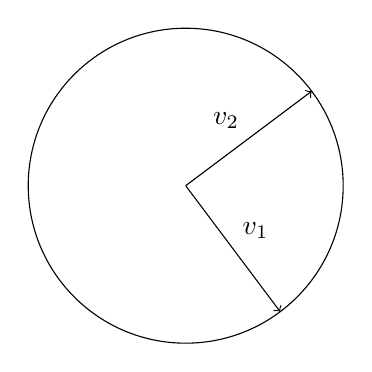
\begin{tikzpicture}[scale=0.4]
        \draw[->] (0,0) -- node[above right] {$v_1$} ++(3,-4);
        \draw[->] (0,0) -- node[above left] {$v_2$} ++(4,3) ;
        \draw (0,0) circle (5);
    \end{tikzpicture}
\end{minipage}
$\xLongrightarrow{\quad f\quad}$
\begin{minipage}[c]{0.3\linewidth}
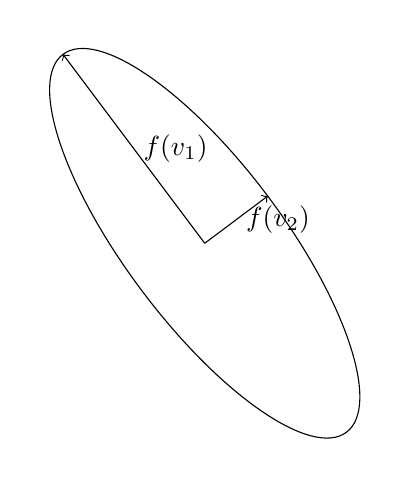
\begin{tikzpicture}[scale=0.4]
        \draw[->] (0,0) -- node[right] {$f(v_1)$} ++(-3*1.5,4*1.5);
        \draw[->] (0,0) -- node[right] {$f(v_2)$} ++(4*0.5,3*0.5);
        \draw[rotate=36.87] (0,0) ellipse (5*0.5 and 5*1.5);
    \end{tikzpicture}
\end{minipage}
\caption{自伴算子的作用}
\label{fig:symmetric-operator}
\end{figure}

接下来,我们考虑自伴算子的范数与谱的关系. 具体来说,设$f$是$V$上的一个自伴算子,那么根据\Cref{thm:symmetric-operator-spectrum},存在一组标准正交基$e_1,\dots,e_n$,使得$f(e_i)=\lambda_i e_i$,$\lambda_i$是特征值(可重复),此时$f$对应的矩阵记为$A$,它是一个对角矩阵. 考虑任何一个向量$x\in V$,它的坐标是$X$,那么
\[
    \norm{f(x)}^2=\norm{AX}^2=\sum_{i=1}^n\lambda_i^2x_i^2.
\]
假设$|\lambda_1|\geq|\lambda_2|\geq\cdots\geq|\lambda_n|$,那么
\[
    |\lambda_n|^2\sum_{i=1}^n x_i^2\leq \sum_{i=1}^n\lambda_i^2x_i^2\leq |\lambda_1|^2\sum_{i=1}^n x_i^2.
\]
因此
\[
    |\lambda_n|\norm{x}\leq \norm{f(x)}\leq |\lambda_1|\norm{x}.
\]
从左到右,等号分别在$x=e_n$和$x=e_1$时取到. 因此,我们得到了

\begin{proposition}\label{prop:symmetric-operator-norm}
    设$V$是一个$n$维内积空间,$f$是$V$上的一个自伴算子,那么
    \[\norm{f}=\max_{\lambda\in\sigma(f)}|\lambda|.\]
    如果最大值在特征值$\lambda_0$取到,其对应单位特征向量是$e_0$,那么$\norm{f(e_0)}=\norm{f}=|\lambda_0|$.
\end{proposition}

最大的特征值模称为算子的\emph{谱半径}\index{谱半径}. 从几何意义来说,谱半径就是算子对应的线性变换对应的线性变换对向量的最大拉伸率. 也可以理解为,将这些基向量画一个球包起来,算子会将这个球映射到一个椭球,这个椭球的最长轴就是谱半径. 例如,对于\Cref{fig:symmetric-operator} 中的算子,谱半径就是$1.5$. 